%% University of Tübingen Academic Poster Template

% Forked from Gemini theme
% https://github.com/anishathalye/gemini

% Required Compiler: LuaLaTeX

\documentclass[final]{beamer}

% ====================
% Packages
% ====================

\usepackage[T1]{fontenc}
\usepackage{lmodern}
\usepackage[size=custom,width=120,height=72,scale=1.0]{beamerposter} % default
% \usepackage[orientation=landscape,size=a0,scale=1.4]{beamerposter} % custom
% scale: scaling factor of all font

\usetheme{gemini}
\usecolortheme{Tuebingen} % Customize in beamercolorthemeTuebingen.sty

\usepackage{graphicx}
\usepackage{booktabs}
\usepackage{tikz}
\usepackage{pgfplots}
\pgfplotsset{compat=1.14}
\usepackage{anyfontsize}

% ====================
% Lengths
% ====================

% If you have N columns, choose \sepwidth and \colwidth such that
% (N+1)*\sepwidth + N*\colwidth = \paperwidth
\newlength{\sepwidth}
\newlength{\colwidth}
\setlength{\sepwidth}{0.025\paperwidth}
\setlength{\colwidth}{0.3\paperwidth}

\newcommand{\separatorcolumn}{\begin{column}{\sepwidth}\end{column}}

% ====================
% Title
% ====================

\title{California Wildfire Risk Prediction and Visualization}

\author{David J. Castrejon \inst{1} \and Connor Wang \inst{2} \and Denys Osmak \inst{3}\\ \and Bhumil Kukadiya \inst{4} \and Dr. Li Liu \inst{4} \and Dr. Mario Giraldo \inst{4} \and Dr. Xunfei Jiang \inst{4} }

\institute [shortinst]{
%\vadjust{\vspace{10pt}}\nolinebreak\hspace{\fill}\linebreak
\inst{1} California State University, Sacramento \samelineand \inst{2} University of California, Los Angeles \samelineand \inst{3}  The University of Texas at Austin \samelineand \inst{4} California State University, Northridge }

% ====================
% Footer (optional)
% ====================

\footercontent{

  \centering 
  REU Site: Applying Data Science on Energy-efficient Cluster Systems and Applications  \hspace{4cm}
  (Email: davidcastrejon@csus.edu, cwang104@g.ucla.edu, denys.osmak@gmail.com, li.liu@csun.edu, mario.giraldo@csun.edu, xunfei.jiang@csun.edu)
 
}
% ====================
% Logo (optional)
% ====================

% use this to include logos on the left and/or right side of the header:
\logoright{
\includegraphics[height=5.5cm]{images/csunlogo.png}}
\logoleft{\includegraphics[height=6cm]{images/nsflogo.png}}
% \logoleft{\includegraphics[height=7cm]{logo2.pdf}}

% ====================
% Body
% ====================

\begin{document}

\begin{frame}[t]
\begin{columns}[t]
\separatorcolumn

\begin{column}{\colwidth}
  
  \begin{block}{Introduction}

    This research aims to investigate the impact of integrating diverse geospatial datasets for training machine-learning models to asses wildfire risk in California. The performance of six machine learning models (Multilayer Perceptron (MLP), Gaussian Naive Bayes (GNB), Support Vector Machine (SVM), Random Forrest (RF), Linear Regression (LR), and K-Nearest Neighbors (KNN)) were analyzed and explored in this project to choose the most accurate model for this task.  Additionally, this research seeks to develop unique data visualization methods to present significant information derived from each of the heterogeneous data indices using the 3D computer graphics software Blender. 
    
    %Overall, The examination of various fire datasets, the use of sophisticated machine learning algorithms, the development of energy-efficient data display techniques, and the development of a user-friendly interface for accessing weather and forecasting data are all included in this research project.

  
  \end{block}

  \begin{alertblock}{Datasets}

    A total of six heterogeneous geospatial remote sensing datasets were selected to be preprocessed, visualized, and fed into machine learning models for wildfire risk prediction. Data was collected for a decade, from 2013-2023.

    \begin{table}
      \centering
      \caption{List of datasets.}
      \begin{tabular}{l c r}
        \toprule
        \textbf{Index} & \textbf{Temporal Freq.} & \textbf{Source} \\
        \midrule
        Enhanced Vegetation Index (EVI) & 16 day & NASA APPEARS \\
        Land Surface Temperature (LST)& 16 day & NASA APPEARS \\
        Thermal Anomalies (TA) & 16 day & NASA APPEARS \\
        Burned Area (BA) & N/A & NASA APPEARS \\
        Average Wind Speed (AWS) & Daily & GHCND\cite{wind} \\ 
        Fire Records & N/A & CAL Fire
        \bottomrule
      \end{tabular}
      % \caption{List of datasets.}
    \end{table}

  \end{alertblock}

  \begin{block}{Methods}

     The input datasets include TIFF format satellite images obtained using the NASA APPEARS tool with each pixel representing an area $ 500m^2 $ in size and weather station wind observations from the Global Historical Climatology Network in .csv format. Given the varying temporal frequency of our data, linear interpolation allowed all datasets to be converted into a daily temporal frequency. The wind data was also converted into TIFF file format by calculating the closest wind observation to each pixel for each day. 

    
    \begin{figure}
    \centering
    \begin{minipage}{0.5\textwidth}
        \centering
        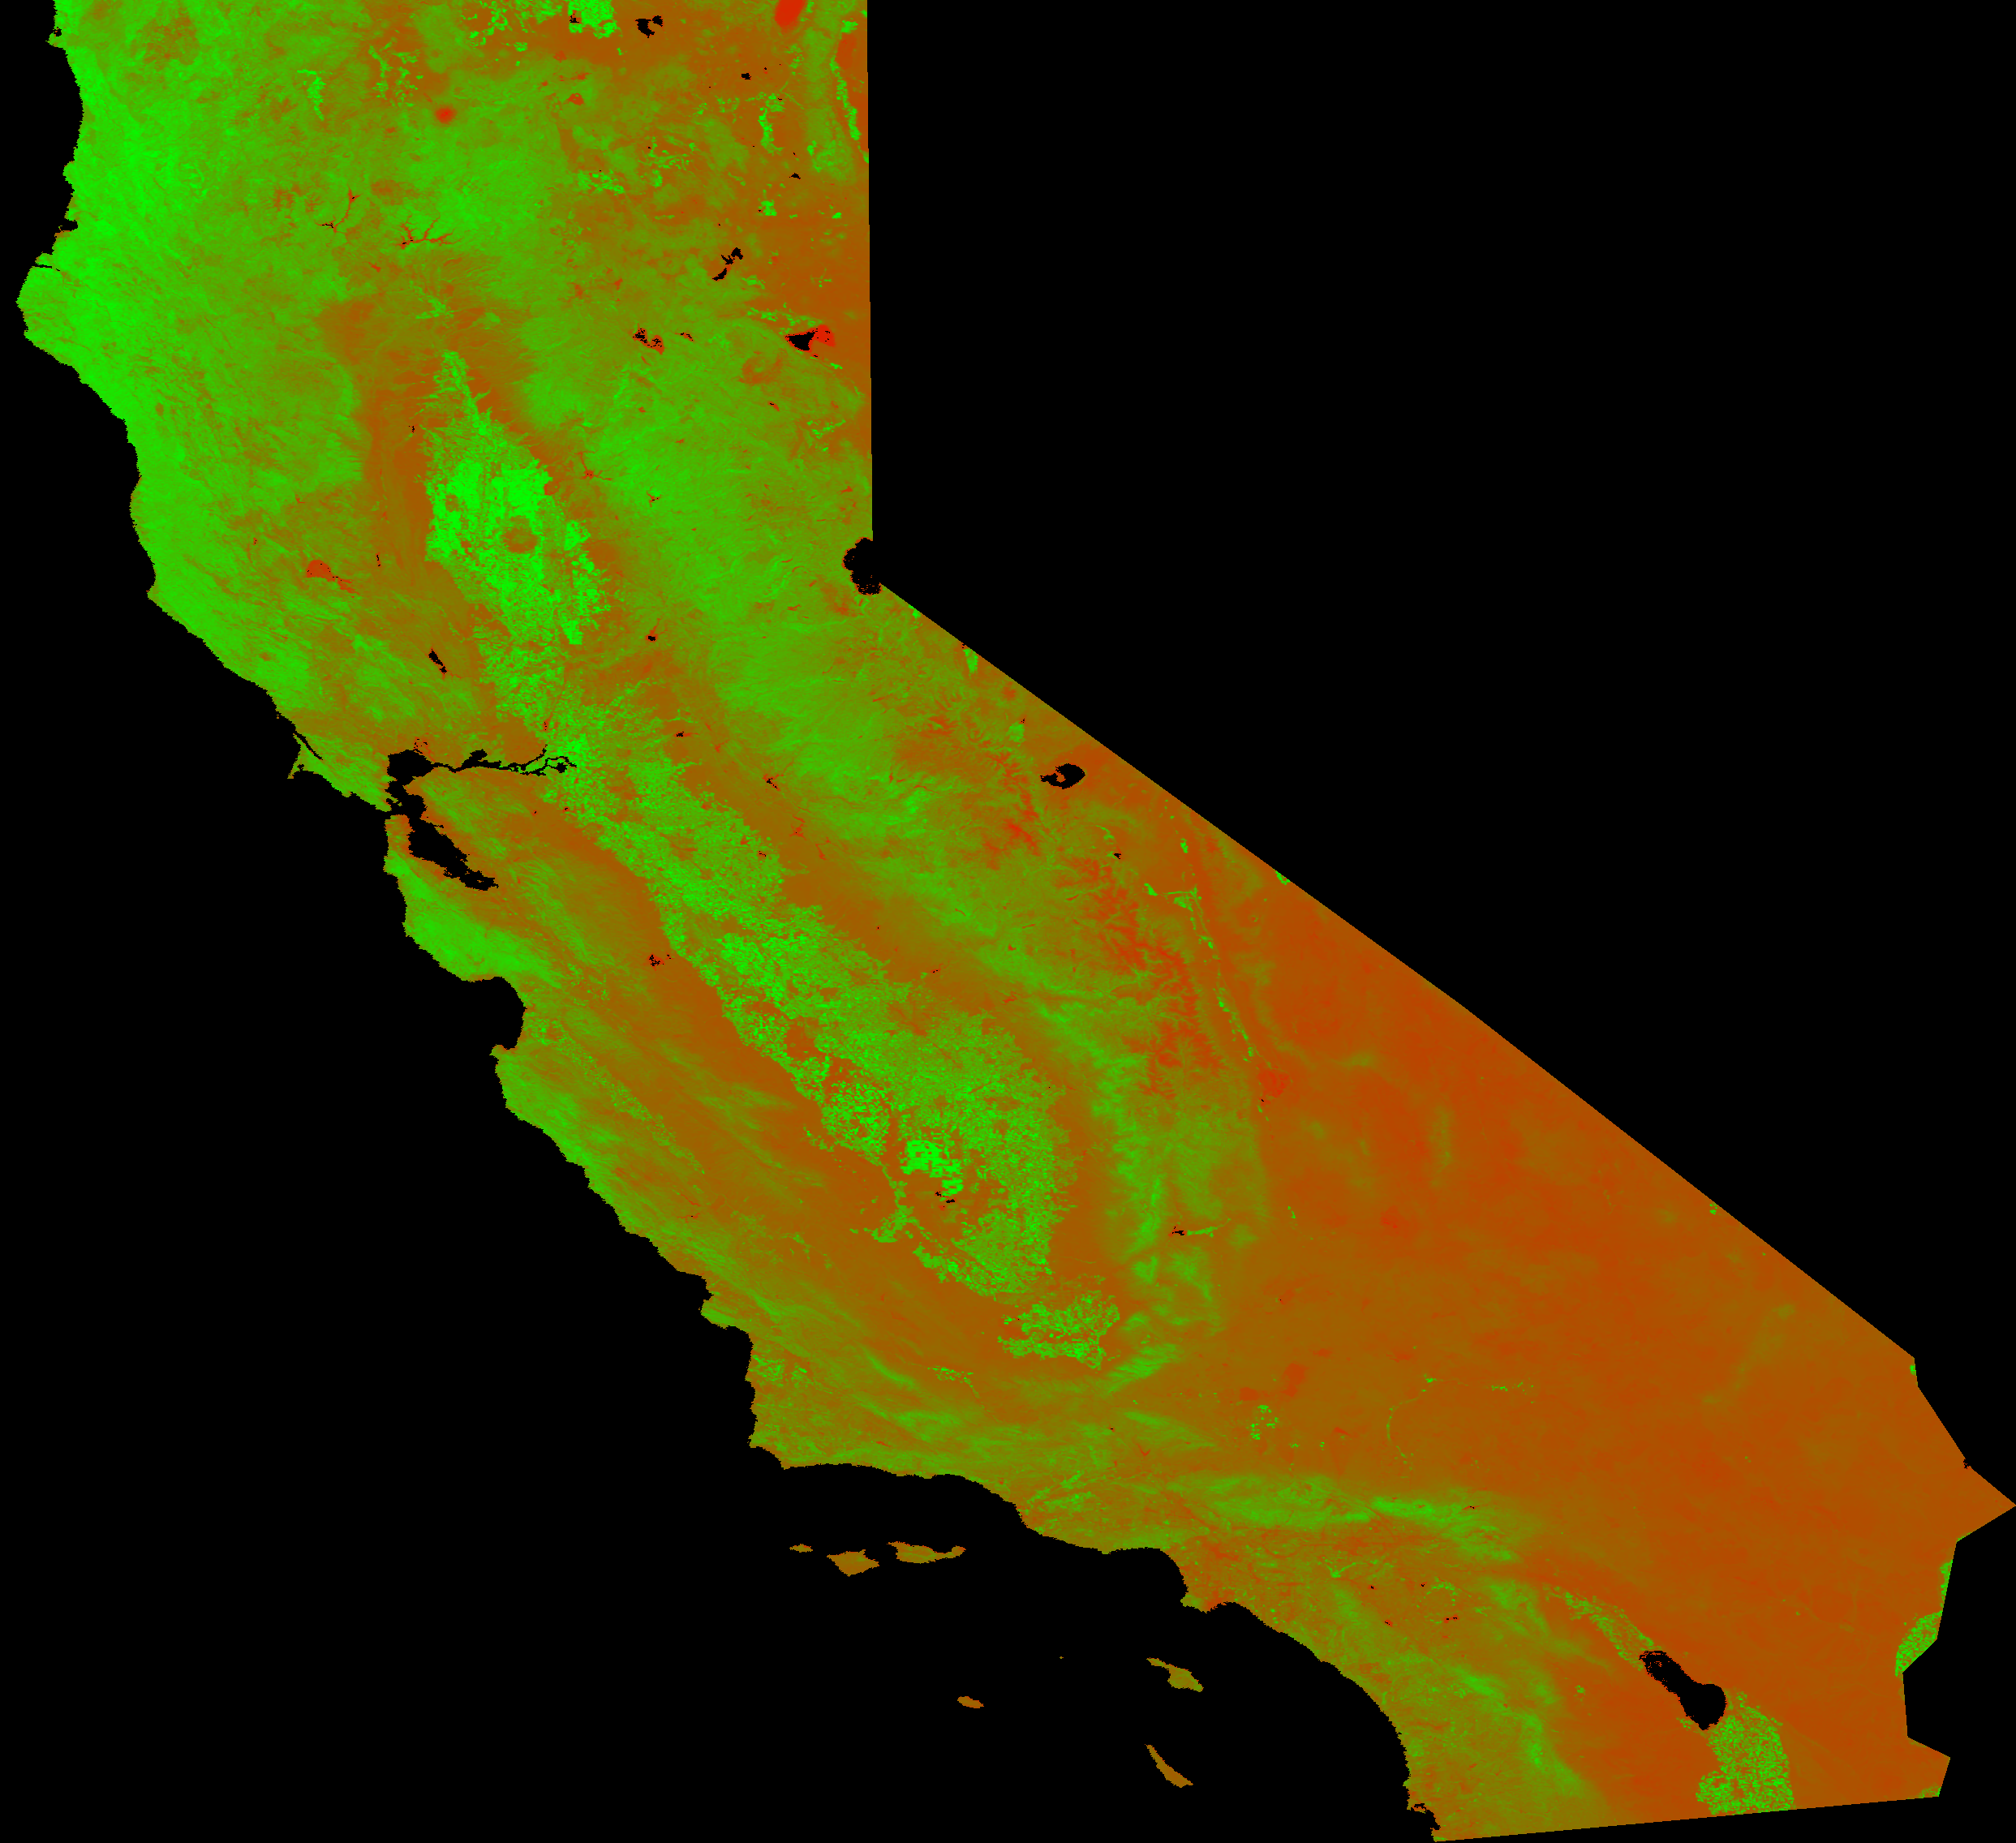
\includegraphics[width=0.75\textwidth]{images/2DCAEVI.png}
        \caption{EVI converted to TIFF file format. Green represents higher EVI.}
        \label{fig:CAEVI.png}
    \end{minipage}%
    \begin{minipage}{0.5\textwidth}
        \centering
        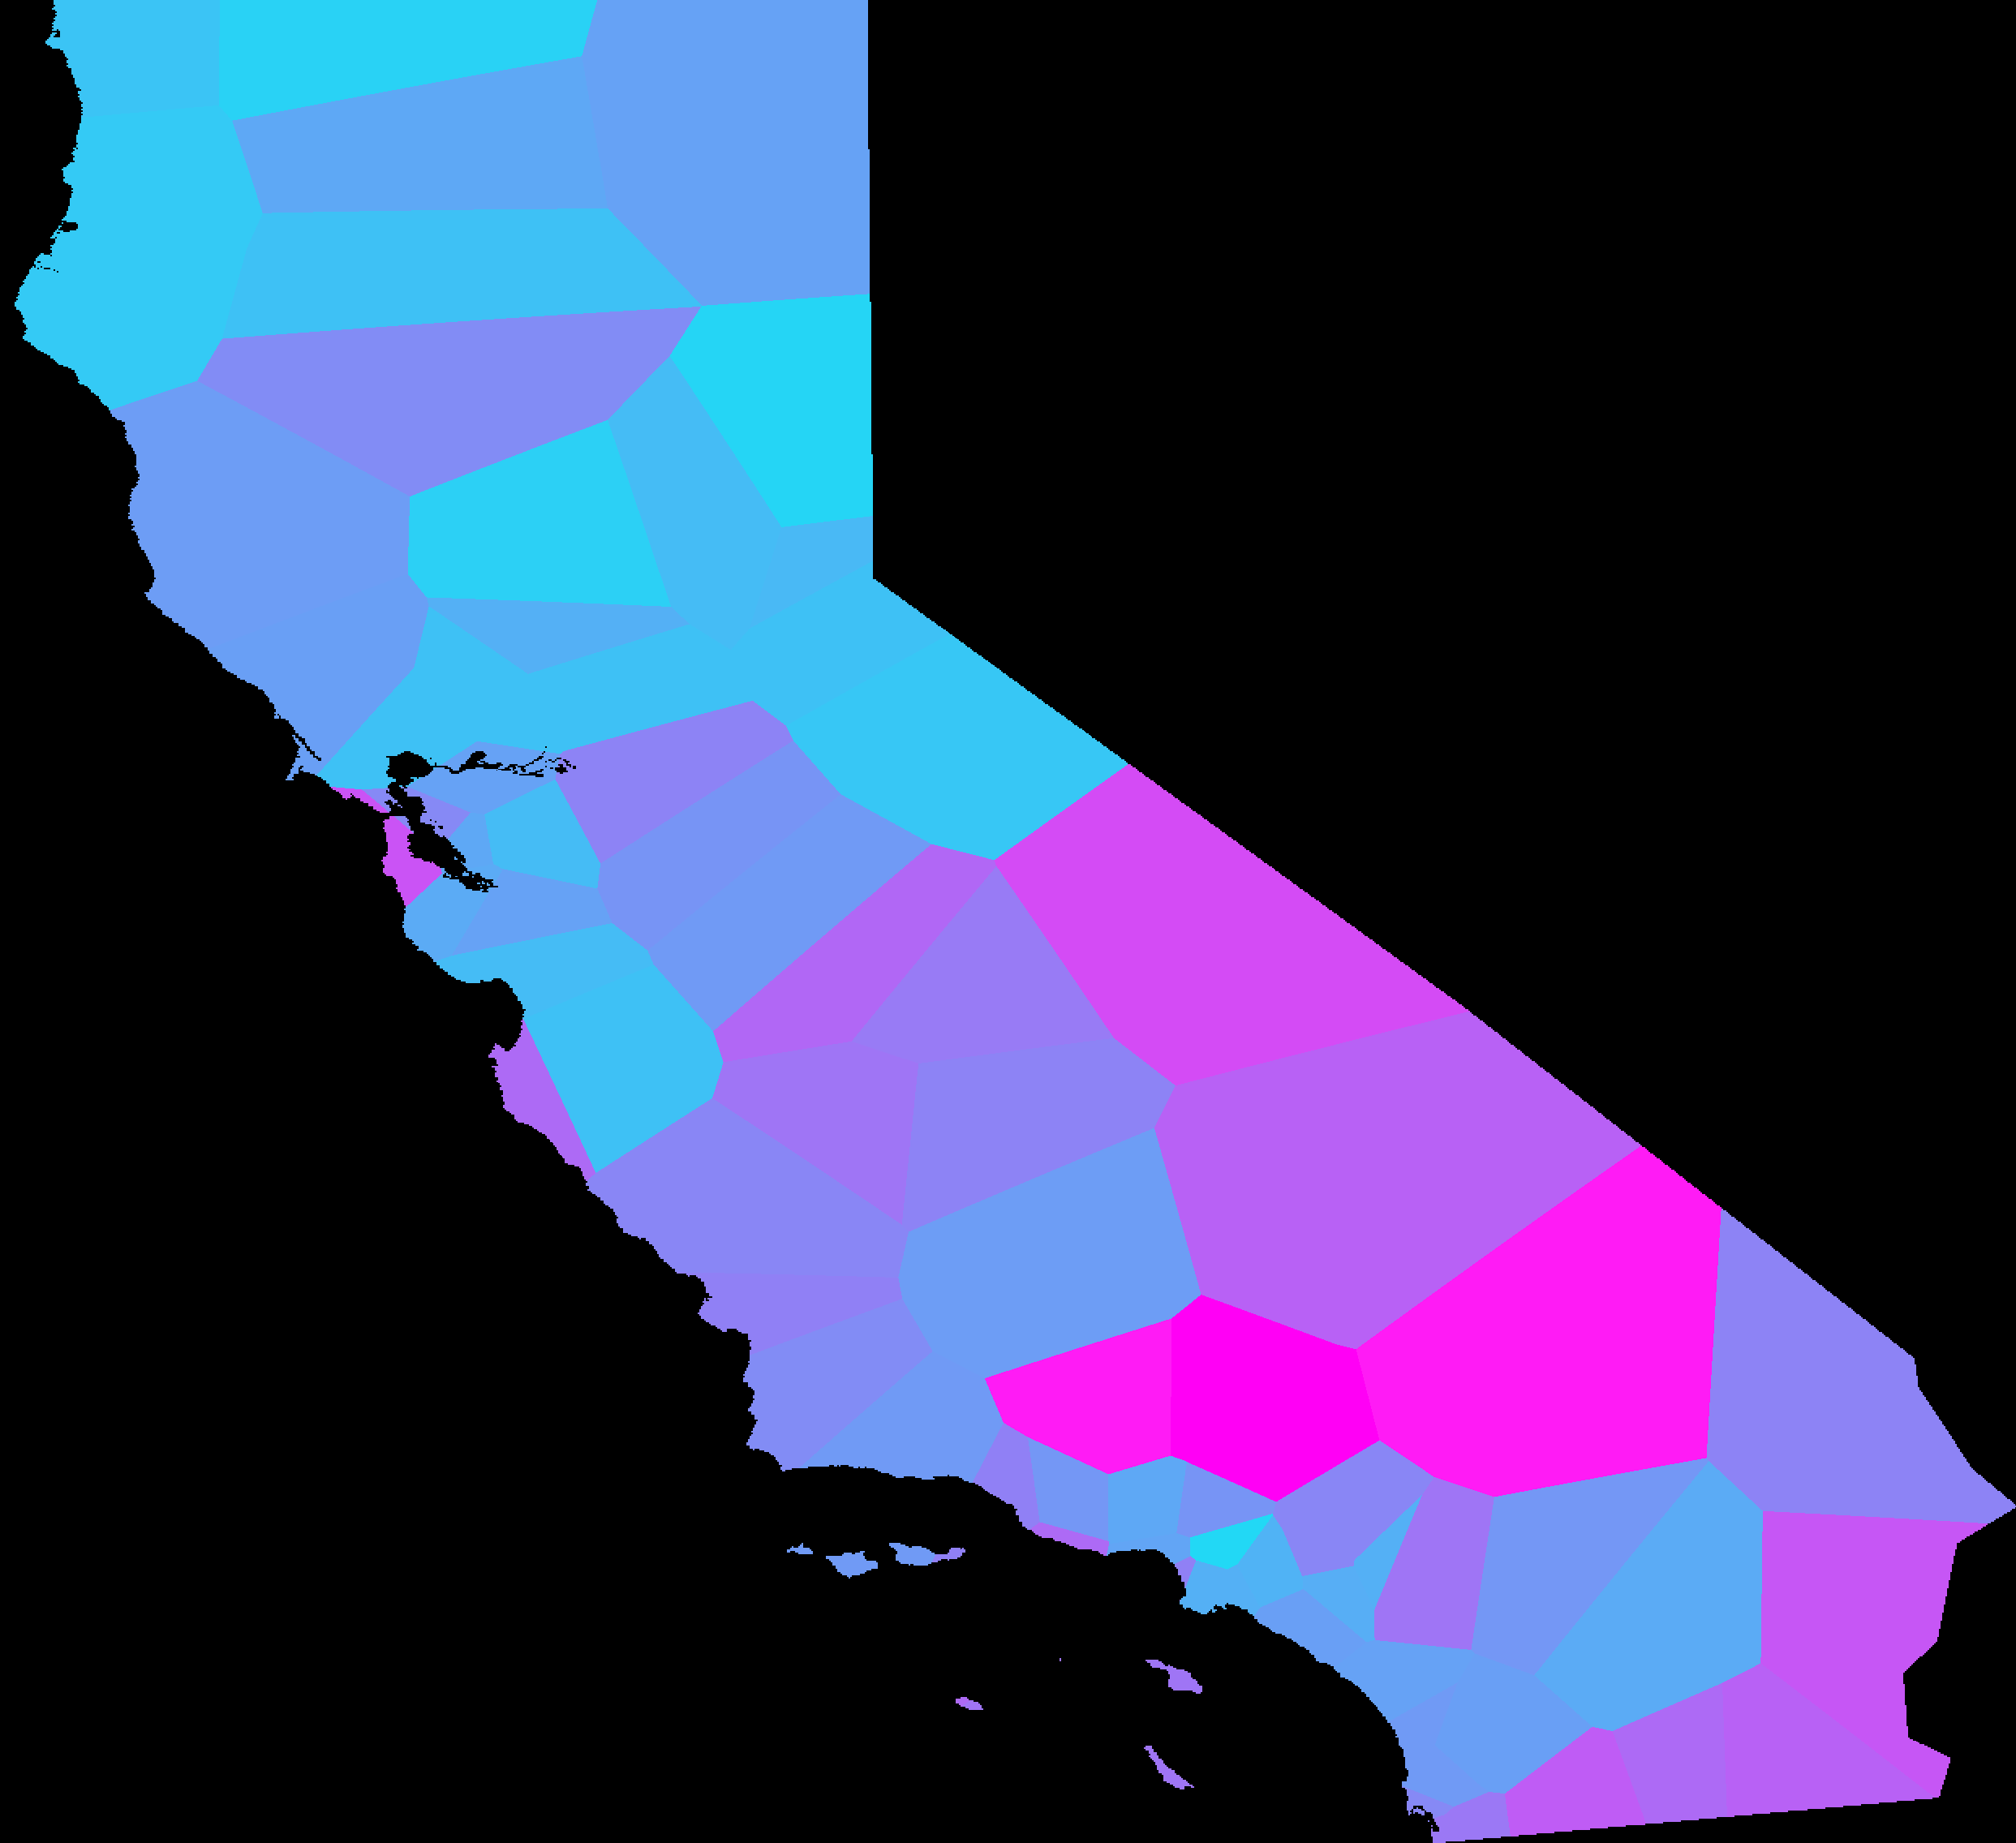
\includegraphics[width=0.75\textwidth]{images/2DCAwind.png}
        \caption{AWS converted to TIFF file format. Pink represents higher wind speeds.}
        \label{fig:2DCAwind.png}
    \end{minipage}
\end{figure}

    An image was generated for every day, for every dataset, totaling over 20,000 images.

  \end{block}

  
\end{column}

\separatorcolumn

\begin{column}{\colwidth}

  \begin{block}{Data Visualizations}

    Blender was used to generate and render 3D visualizations of five of the datasets. These visualizations add a layer of depth, in addition to color, which emphasizes features which may be difficult to notice in a 2D visualization. Animations were also produced which allowed for the visualization of datasets over the 10-year period.
    \vspace{1cm}
    \begin{figure}
        \centering
        \begin{minipage}{0.5\textwidth}
            \centering
            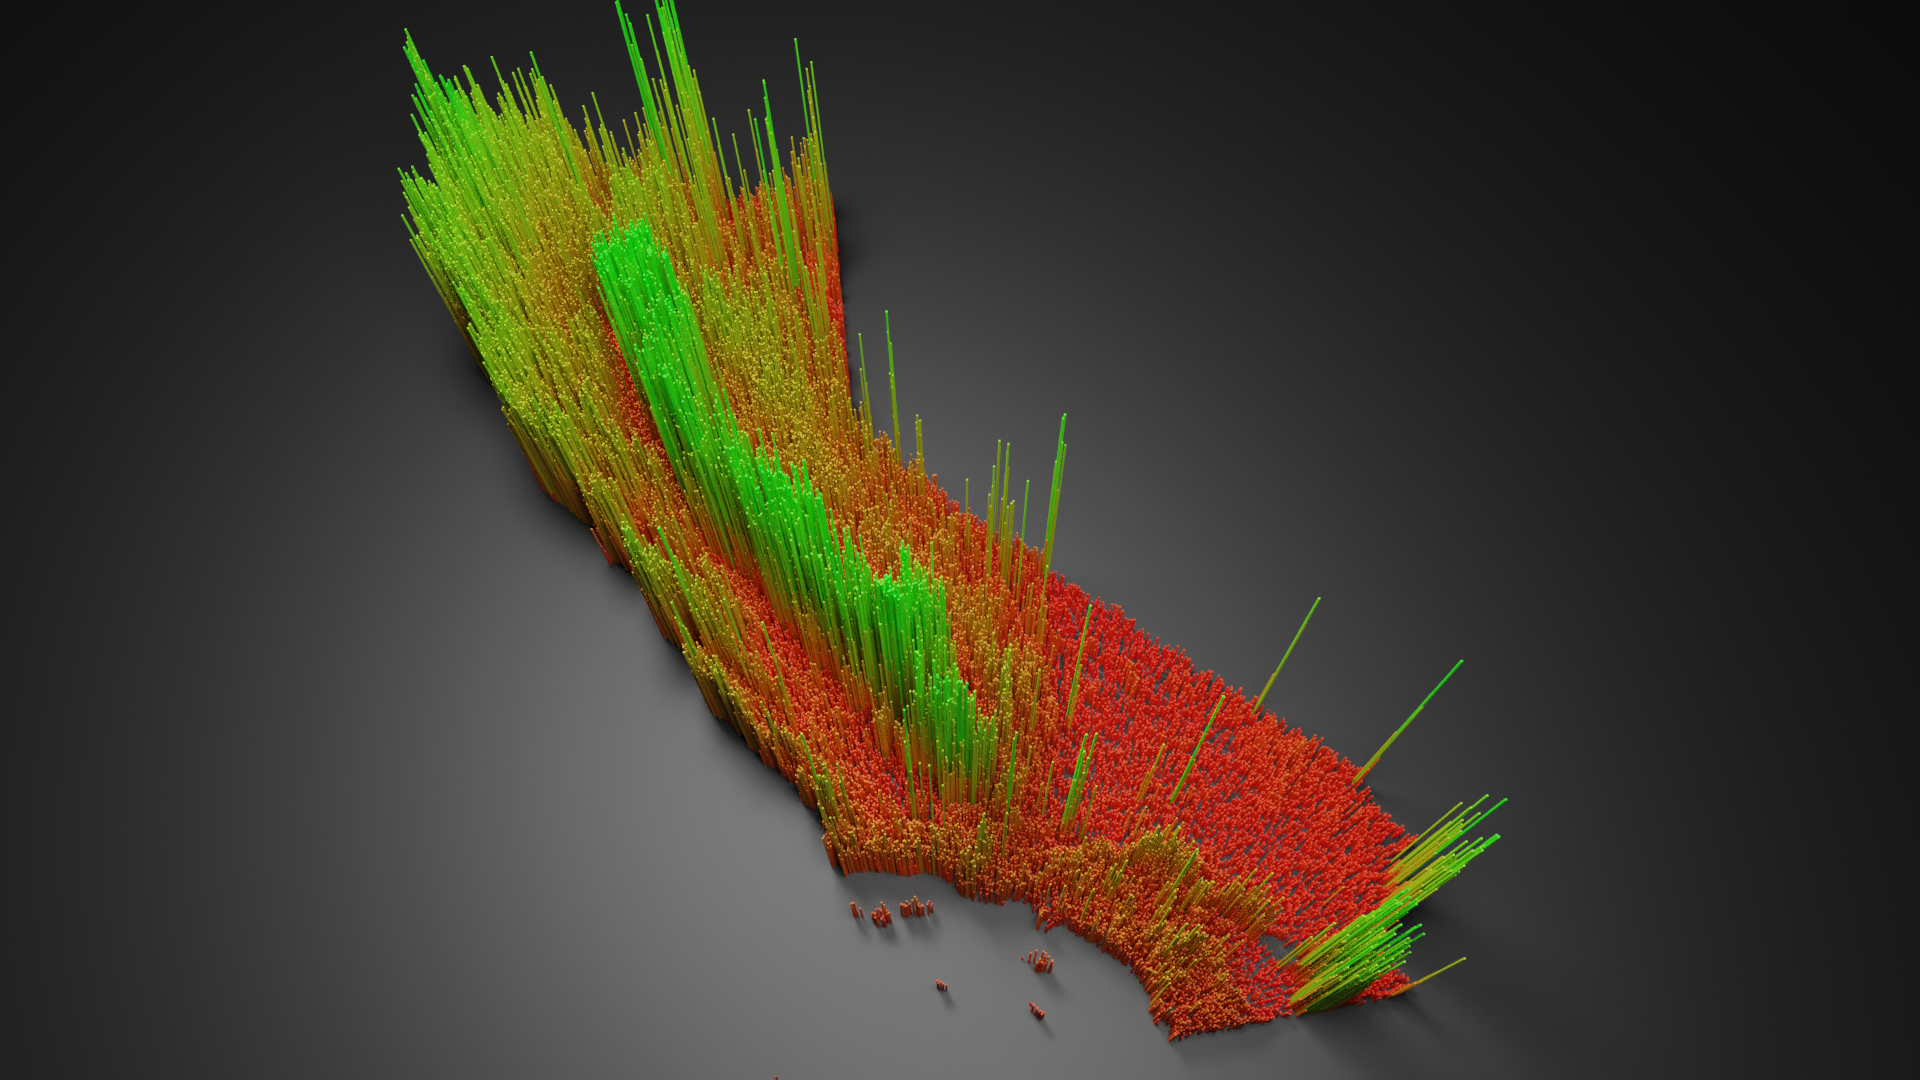
\includegraphics[width=0.95\textwidth]{images/CAEVI.png}
            \caption{Enhanced Vegetation Index Visualization.}
            \label{fig:CAEVI.png}
        \end{minipage}%
        \begin{minipage}{0.5\textwidth}
            \centering
            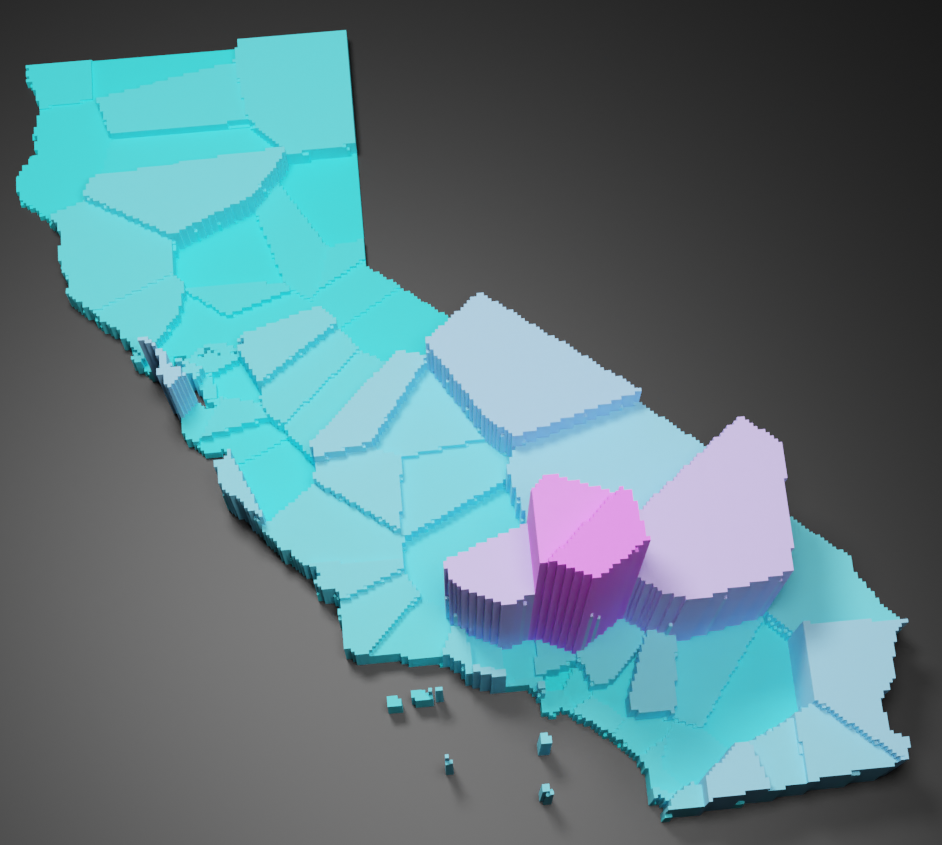
\includegraphics[width=0.95\textwidth]{images/wind.png}
            \caption{Average Wind Speed Visualization.}
            \label{fig:wind.png}
        \end{minipage}
    \end{figure}

  \end{block}

  \begin{block}{Data Preprocessing}

    For the purposes of the machine learning model, only areas which have been previously burned were analyzed for fire-proneness. All our datasets were filtered by Burned Area, only extracting pixels which have previously been burned in the past 10 years, about 4-5 \% of the total data.
    
    Areas of high fire risk were defined as any section of land at a certain point in time in which a fire occurred in the next 30 days. Each pixel over the 10 years was classified as either fire-prone or not fire-prone, and placed in a CSV file along with EVI, LST, AWS, and TA values. Finally, outliers were removed. The final CSV file contained over a hundred million data points.
    \vspace{1cm}
    \begin{figure}
        \centering
        \begin{minipage}{0.5\textwidth}
            \centering
            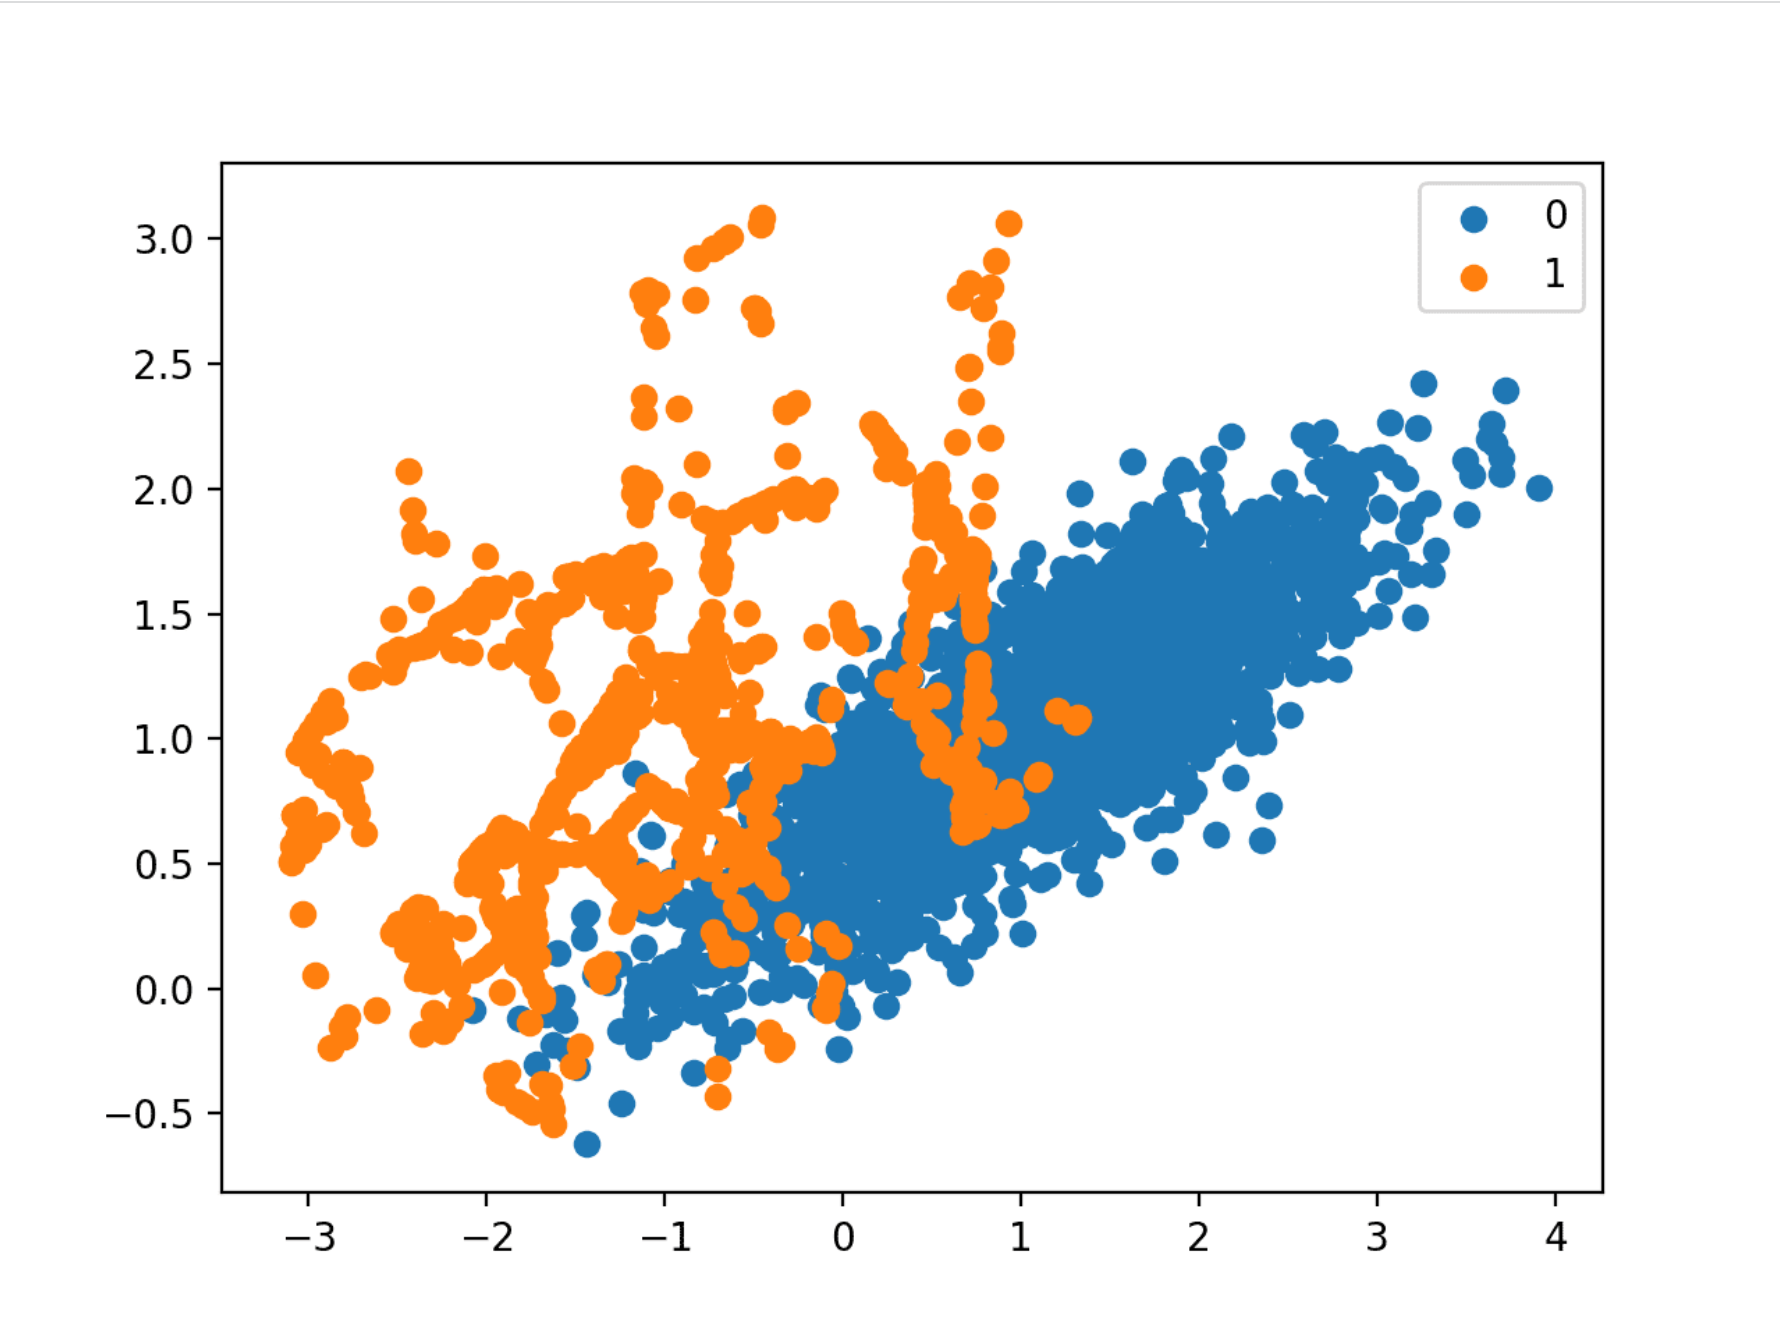
\includegraphics[width=0.95\textwidth]{images/SMOTE.png}
            \caption{SMOTE Example. The minority class (orange) has been oversampled with SMOTE.}
            \label{fig:CAEVI.png}
        \end{minipage}%
        \begin{minipage}{0.5\textwidth}
            \centering
            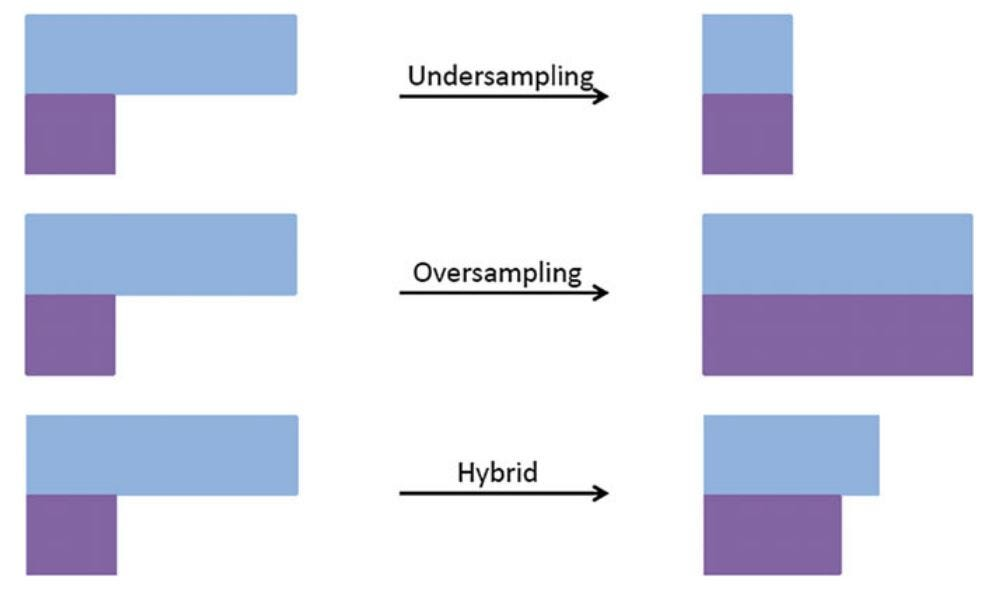
\includegraphics[width=0.95\textwidth]{images/UnderOver.jpeg}
            \caption{Oversampling/Undersampling Example}
            \label{fig:wind.png}
        \end{minipage}
    \end{figure}
    
  \end{block}

\end{column}

\separatorcolumn

\begin{column}{\colwidth}

  \begin{exampleblock}{Machine Learning Models}
    The task of classifying land areas as either fire-prone or not fire-prone takes the form of a binary classification problem. In testing different models, the method which produced the best results was the Multi-Layer Perceptron (MLP) model. Hyperparameters were tuned using a grid search method, testing hundreds of models with varying hidden layers and nodes, solvers, and activation functions. 
    
    Early into model training, an issue that became obvious was the imbalance of fire-prone data to not fire-prone data, a ratio of about 1:32000. This would cause early models to classify all areas as not fire-prone. To fix this, different oversampling and undersampling approaches were tested, as well as different fire-prone to not fire-prone data ratios.
    \vspace{-1em}
    \begin{figure}
        \centering
        \begin{minipage}{0.5\textwidth}
            \centering
            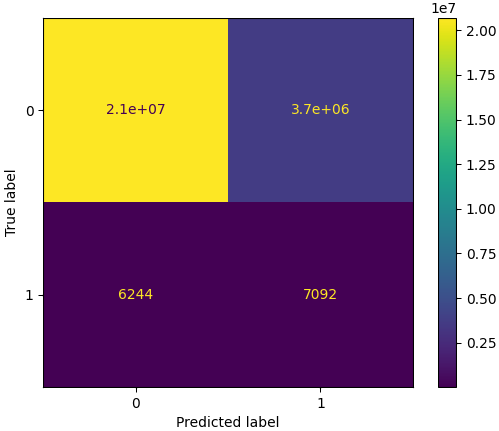
\includegraphics[width=1\textwidth]{images/MLP.png}
            \caption{Multi-Layer Perceptron}
            \label{fig:CAEVI.png}
        \end{minipage}%
        \begin{minipage}{0.5\textwidth}
            \centering
            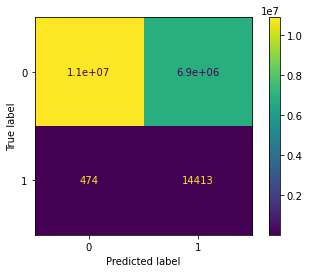
\includegraphics[width=1\textwidth]{images/GNB.png}
            \caption{Guassian Naive Bayes}
            \label{fig:wind.png}
        \end{minipage}
    \end{figure}
    
  \end{exampleblock}

  \begin{block}{Conclusion}

    Utilization of 3D computer graphics software like Blender can led to unique visualizations and animations that have potential for expressing previously unseen visualizations of heterogeneous geospatial datasets. In addition, the machine learning models showed improvement in wildfire prediction upon implementing oversampling methods such as SMOTE. The restriction of having 1 fire measurement for every 32,000 non fire measurement led to this issue and further work needs to be done to further develop the machine learning models.

    Future research on overcoming the imbalanced dataset of fire/no fire data and including more relevant data indices could allow machine learning models to make highly accurate fire risk predictions, potentially saving the lives of millions. In addition, there is a glaring lack of easily accessible online geospatial datasets open to the general population. Updating online geospatial datasets and publishing more easily accessible data can be pivotal in the fight against climate change, as well as inspire others to do their best to save our planet. 

  \end{block}

  \begin{block}{References}
    \vspace{-0.2cm}
    \nocite{*}
    \footnotesize{\bibliographystyle{plain}\bibliography{poster}}

%     @article{appears,
%   author = {“Appeears,” NASA, https://appeears.earthdatacloud.nasa.gov/.}
% }

% @article{fire,
%   author = { “Calfire,” Cal FIRE, https://www.fire.ca.gov/.}
% }

  \end{block}
  \begin{block}{Acknowledgements}
    This project is supported by the National Science Foundation under Grant CNS-2244391.
  \end{block}
\end{column}

\separatorcolumn
\end{columns}

\end{frame}

\end{document}
